\chapter{การติดตั้ง ใช้งานจริง และการตรวจสอบความใช้ได้ของวิธี}
\label{chap:ch06}

\section*{แผนบริหารการสอนประจำบทที่ 6}
\addcontentsline{toc}{section}{แผนบริหารการสอนประจำบทที่ 6}

\begin{tcolorbox}[
    enhanced, breakable,
    colback=white, colframe=rbruNavy,
    fonttitle=\bfseries\color{white},
    title={1. หัวข้อเนื้อหาประจำบท},
    arc=1.5mm, boxrule=0.8pt, leftrule=3.5mm
]
\begin{enumerate}
    \item ขั้นตอนการคอมไพล์และติดตั้งแอปพลิเคชันลงบนสมาร์ตโฟนผ่าน ADB
    \item การเชื่อมต่อสายสัญญาณและการใช้งานแอปพลิเคชันร่วมกับหัววัดจริง
    \item ระเบียบวิธีตรวจสอบความใช้ได้ของวิธีตามมาตรฐานสากล EURACHEM / ISO 17025
    \item การทดสอบเปรียบเทียบในแปลงปลูกทุเรียนจริง 30 แปลง (จันทบุรี-ตราด)
    \item การวิเคราะห์สถิติทดสอบสมมติฐานและความสอดคล้องของแบลนด์-อัลต์แมน
\end{enumerate}
\end{tcolorbox}

\begin{tcolorbox}[
    enhanced, breakable,
    colback=white, colframe=rbruNavy,
    fonttitle=\bfseries\color{white},
    title={2. วัตถุประสงค์เชิงพฤติกรรม},
    arc=1.5mm, boxrule=0.8pt, leftrule=3.5mm
]
เมื่อศึกษาบทเรียนนี้จบแล้ว ผู้เรียนสามารถ
\begin{enumerate}
    \item ติดตั้งและเปิดใช้งานแอปพลิเคชัน Release APK บนสมาร์ตโฟนแอนดรอยด์ได้สำเร็จ
    \item ดำเนินการทดสอบความแม่น (%Bias) และความเที่ยง (%RSD) ตามมาตรฐาน EURACHEM ได้อย่างถูกต้อง
    \item วิเคราะห์ผลการทดสอบ Paired Samples t-test และอธิบายค่า p-value ทางสถิติได้อย่างแม่นยำ
    \item สร้างและตีความแผนภาพความสอดคล้องของแบลนด์-อัลต์แมนได้อย่างสมบูรณ์
\end{enumerate}
\end{tcolorbox}

\begin{tcolorbox}[
    enhanced, breakable,
    colback=white, colframe=rbruNavy,
    fonttitle=\bfseries\color{white},
    title={3. วิธีสอนและกิจกรรมการเรียนการสอน},
    arc=1.5mm, boxrule=0.8pt, leftrule=3.5mm
]
\begin{enumerate}
    \item การสาธิตการเชื่อมต่อหัววัดเซนเซอร์จริงเข้ากับสมาร์ตโฟนผ่านสายแปลง USB OTG
    \item กิจกรรมฝึกปฏิบัติการเก็บข้อมูลดินและส่งออกไฟล์ตารางคำนวณ Excel
    \item การฝึกวิเคราะห์ข้อมูลทางสถิติด้วยโปรแกรมคำนวณและการอภิปรายผลร่วมกัน
\end{enumerate}
\end{tcolorbox}

\begin{tcolorbox}[
    enhanced, breakable,
    colback=white, colframe=rbruNavy,
    fonttitle=\bfseries\color{white},
    title={4. สื่อการเรียนการสอน},
    arc=1.5mm, boxrule=0.8pt, leftrule=3.5mm
]
\begin{enumerate}
    \item ชุดเครื่องมือวัด JC AI Detector พร้อมหัววัด 8-in-1 และสายแปลง Type-C
    \item สารละลายมาตรฐานบัฟเฟอร์ NIST (pH 4.01, 7.00) และสารละลายมาตรฐาน KCl
    \item ตารางชุดข้อมูลผลการตรวจวัดดินจริง 30 แปลงตัวอย่าง
\end{enumerate}
\end{tcolorbox}

\begin{tcolorbox}[
    enhanced, breakable,
    colback=white, colframe=rbruNavy,
    fonttitle=\bfseries\color{white},
    title={5. การวัดและประเมินผล},
    arc=1.5mm, boxrule=0.8pt, leftrule=3.5mm
]
\begin{enumerate}
    \item การประเมินทักษะการปฏิบัติการใช้เครื่องมือวัดในสนามทดลองจริง
    \item การตรวจรายงานผลการตรวจสอบความใช้ได้ของวิธีและการวิเคราะห์ทางสถิติ
    \item การสังเกตความรับผิดชอบและความร่วมมือในการทำงานภาคสนาม
\end{enumerate}
\end{tcolorbox}

\clearpage

% ==============================================================================
% ภาพประกอบเกริ่นนำประจำบทที่ 6 (Introductory Infographic)
% ==============================================================================
\begin{figure}[H]
\centering
\begin{tikzpicture}[
    box/.style={rectangle, rounded corners=2mm, draw=rbruNavy, line width=1.0pt, fill=white, drop shadow={shadow xshift=1pt, shadow yshift=-1.5pt, opacity=0.15}, align=center, inner sep=5pt},
    header/.style={rectangle, rounded corners=1.5mm, draw=rbruNavy, fill=rbruNavy, text=white, font=\bfseries\scriptsize, align=center, inner sep=3.5pt},
    arrow/.style={-{Stealth[scale=1.0]}, line width=1.1pt, draw=rbruBlue}
]
    % ขั้นตอนที่ 1: การคอมไพล์
    \node[box, fill=cyan!10, minimum width=3.2cm] (build) {
        \textbf{การสร้างไฟล์ติดตั้ง}\\[2pt]
        \footnotesize
        $\bullet$ Flutter Build APK\\
        $\bullet$ Release Optimization\\
        $\bullet$ ProGuard / Shrinking
    };
    \node[header, above=2pt of build] {1. ติดตั้ง \& คอมไพล์};

    % ขั้นตอนที่ 2: ติดตั้งบนอุปกรณ์
    \node[box, fill=rbruGold!12, minimum width=3.2cm, right=0.8cm of build] (deploy) {
        \textbf{การลงสู่สมาร์ตโฟน}\\[2pt]
        \footnotesize
        $\bullet$ ADB Streamed Install\\
        $\bullet$ Android USB Permissions\\
        $\bullet$ OTG Auto-Detection
    };
    \node[header, fill=rbruGold!90!black, above=2pt of deploy] {2. การติดตั้งฮาร์ดแวร์};

    % ขั้นตอนที่ 3: ตรวจสอบความใช้ได้ EURACHEM
    \node[box, fill=green!10, minimum width=3.4cm, right=0.8cm of deploy] (valid) {
        \textbf{เกณฑ์ EURACHEM}\\[2pt]
        \footnotesize
        $\bullet$ ความถูกต้อง (\%Bias $< 5\%$)\\
        $\bullet$ ความเที่ยง (\%RSD $< 3\%$)\\
        $\bullet$ Paired t-test ($p > 0.05$)
    };
    \node[header, fill=green!60!black, above=2pt of valid] {3. การตรวจความใช้ได้};

    % ขั้นตอนที่ 4: การนำไปใช้ในแปลงจริง
    \node[box, fill=purple!10, minimum width=3.2cm, right=0.8cm of valid] (field) {
        \textbf{การวิเคราะห์แปลงจริง}\\[2pt]
        \footnotesize
        $\bullet$ สวนทุเรียนจันทบุรี\\
        $\bullet$ Bland-Altman $96.7\%$\\
        $\bullet$ ลดต้นทุน 1.8 หมื่น/ไร่
    };
    \node[header, fill=purple!70!black, above=2pt of field] {4. การประยุกต์ใช้};

    \draw[arrow] (build) -- (deploy);
    \draw[arrow] (deploy) -- (valid);
    \draw[arrow] (valid) -- (field);
\end{tikzpicture}
\caption{ผังกระบวนการคอมไพล์ ติดตั้งลงบนสมาร์ตโฟน และขั้นตอนการตรวจสอบความใช้ได้ของวิธีตามมาตรฐานสากล}
\label{fig:ch06_validation_pipeline}
\end{figure}

\section{ขั้นตอนการคอมไพล์และติดตั้งลงสมาร์ตโฟนผ่าน ADB}

ผู้พัฒนาสามารถคอมไพล์และส่งไฟล์ติดตั้งแอปพลิเคชันเข้าสู่สมาร์ตโฟนแอนดรอยด์ได้โดยตรงผ่านคำสั่ง

\begin{codebox}[title={คำสั่งคอมไพล์และติดตั้งผ่านเทอร์มินัล}]
\begin{lstlisting}[language=bash]
# 1. นำเข้า dependencies ทั้งหมด
flutter pub get

# 2. รันชุดทดสอบความถูกต้องของโมเดลและการคำนวณ
flutter test

# 3. คอมไพล์ไฟล์ติดตั้ง Release APK
flutter build apk --release

# 4. ติดตั้งเข้าสู่สมาร์ตโฟนที่เชื่อมต่อผ่านสาย USB
adb install -r build/app/outputs/flutter-apk/app-release.apk

# 5. สั่งให้แอปพลิเคชันเปิดทำงานบนหน้าจอทันที
adb shell am start -n com.agriphysics.soil_app/com.agriphysics.soil_app.MainActivity
\end{lstlisting}
\end{codebox}

\begin{figure}[H]
\centering
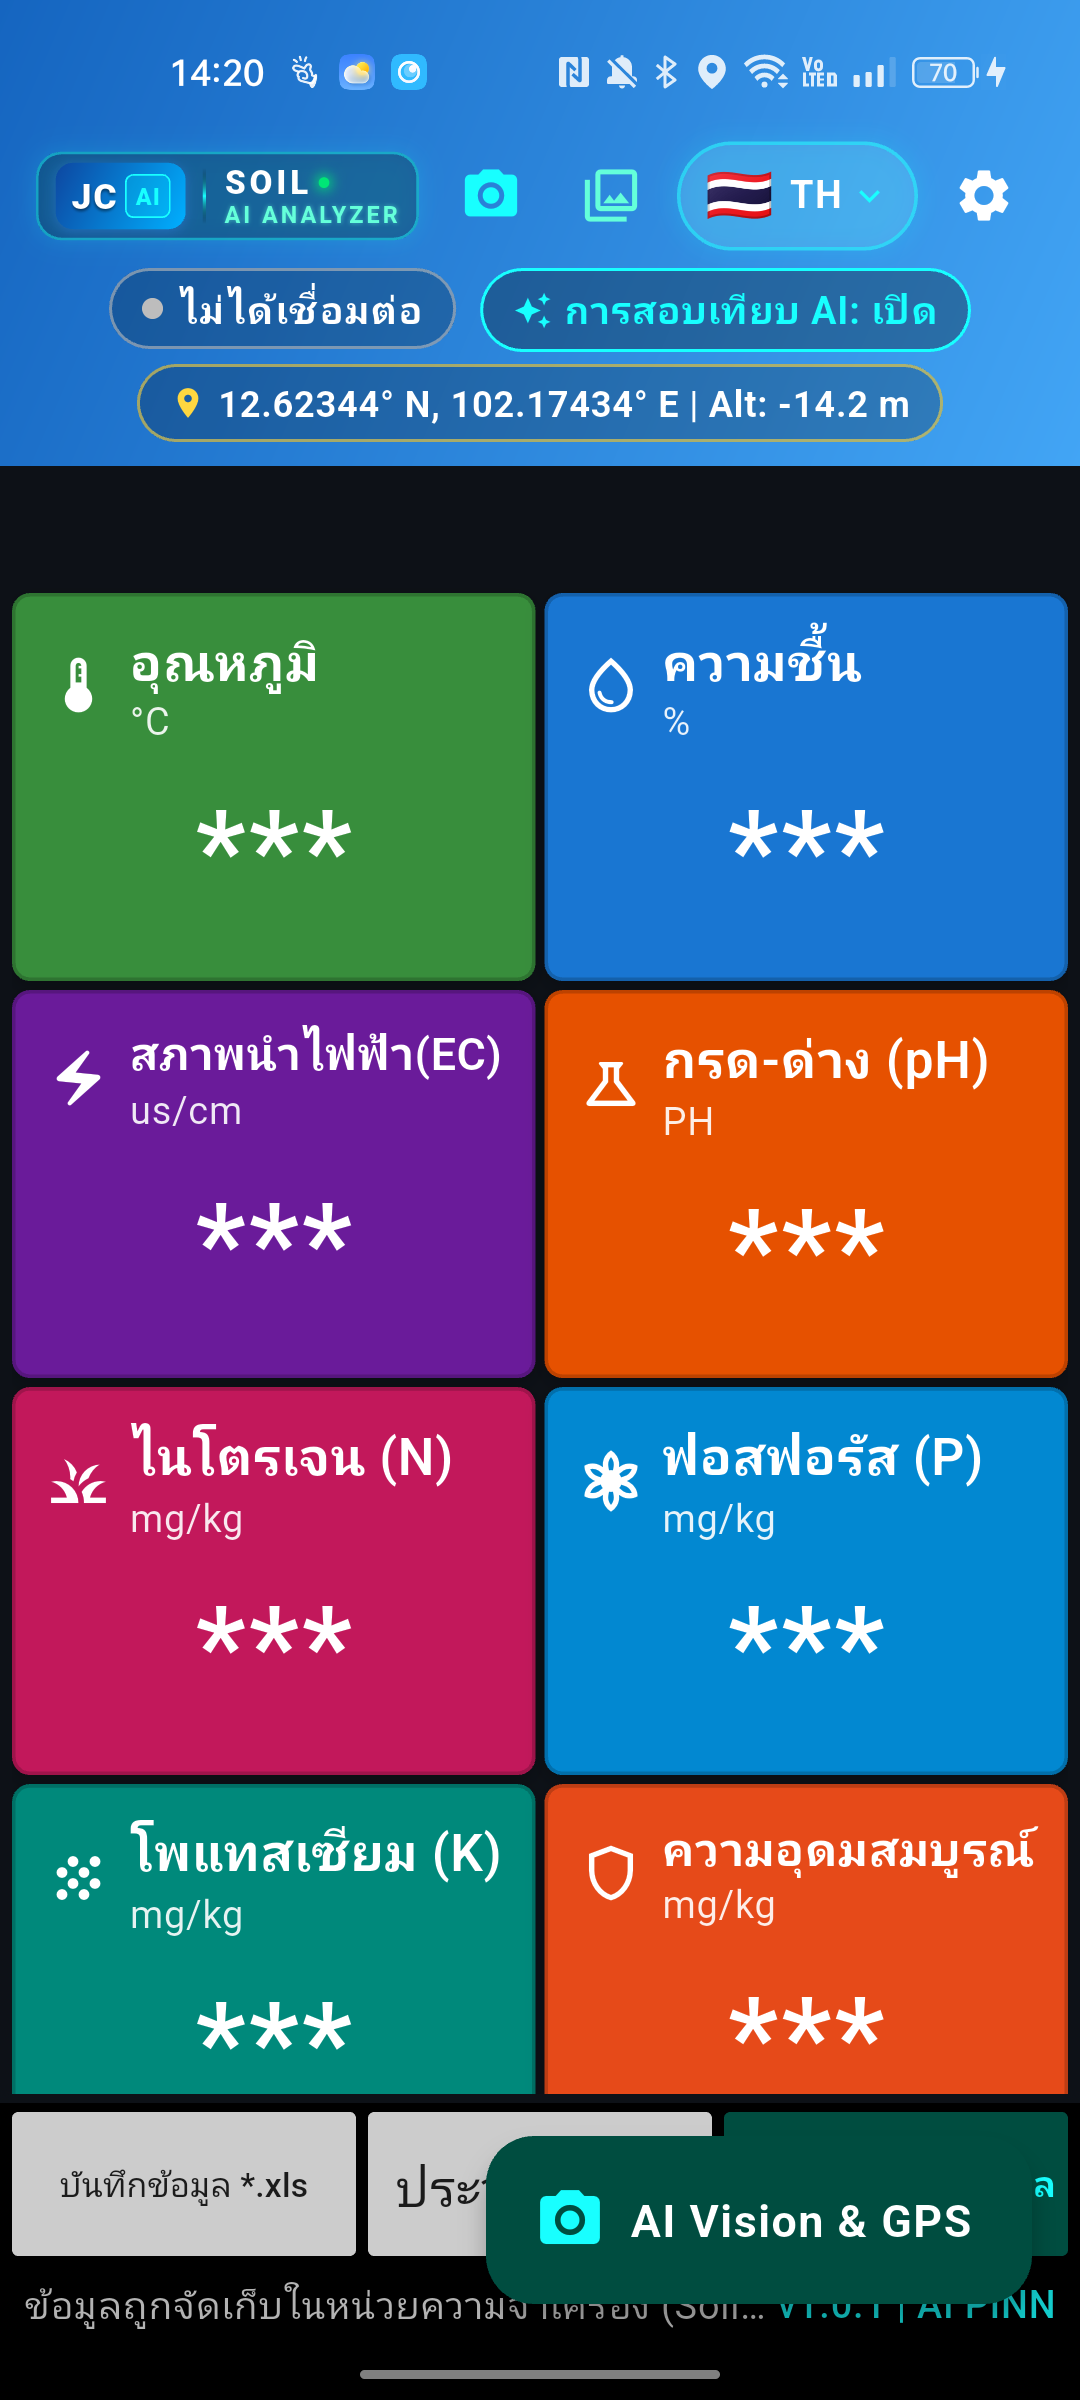
\includegraphics[width=0.48\textwidth]{figures/app_dashboard_live.png}
\caption{หน้าจอแดชบอร์ดหลักของแอปพลิเคชัน JC AI SOIL ANALYZER บนสมาร์ตโฟนจริง พร้อมโลโก้แบรนด์ 2 คอลัมน์ แถบสถานะ GPS และป้ายธงชาติสลับภาษา}
\label{fig:app_ui_screen}
\end{figure}

\section{สถาปัตยกรรมแถบสถานะส่วนหัว 2 คอลัมน์ และระบบปฐพีวิทยาไร้การล้นจอ}

แถบหัวเรื่องของแอปพลิเคชัน (\texttt{StatusHeader}) และแผ่นสรุปผลปฐพีวิทยา (\texttt{AgronomicSummarySheet}) ได้รับการปรับปรุงโครงสร้างสถาปัตยกรรมใหม่เพื่อแก้ปัญหาข้อมูลล้นจอและจัดระเบียบการใช้งาน:
\begin{enumerate}
    \item \textbf{โครงสร้างแถบสถานะส่วนหัว 2 คอลัมน์ (Two-Column StatusHeader):}
    \begin{itemize}
        \item \textbf{คอลัมน์ซ้าย:} การ์ดโลโก้ทรงสูงกรอบเขียวนีออน (\texttt{\#00E676}) จัดวางแนวตั้ง ประกอบด้วย แบดจ์แบรนด์ \textbf{JC AI}, เส้นแบ่งเรืองแสง, ข้อความ \textbf{SOIL} พร้อมจุดมรกต และคำบรรยาย \textbf{AI ANALYZER} โดยยืดความสูงเต็มพื้นที่คอลัมน์ขวาด้วย \texttt{IntrinsicHeight}
        \item \textbf{คอลัมน์ขวา (3 แถว):} แถวที่ 1 รวมปุ่มเครื่องมือ [กล้อง], [คลังภาพ], [ปุ่มสลับภาษา TH/EN/ZH] และ [ปุ่มวงกลมการตั้งค่าสี Dark Teal \texttt{\#0B556A}] / แถวที่ 2 รวมการ์ดสถานะการเชื่อมต่อ USB และการสอบเทียบ AI / แถวที่ 3 แถบพิกัดดาวเทียม (Lat. Long. Alt.) เต็มความกว้าง
    \end{itemize}
    \item \textbf{ระบบประเมินปฐพีวิทยาและโครงสร้าง 2 แท็บ (Dual-Tab Soil Diagnostics):}
    \begin{itemize}
        \item \textbf{ดัชนีสุขภาพดิน (Composite Soil Health Score 0--100):} แสดงคะแนนภาพรวมของแปลงดินพร้อมวงกลมสถานะและตาราง Mini Status Chips 4 มิติ
        \item \textbf{แท็บ 1 (ข้อเสนอแนะ \& แผนปรับปรุงดิน):} คำแนะนำเชิงปริมาณเฉพาะทาง ได้แก่ อัตราปูนโดโลไมต์ปรับค่า pH (200--300 กก./ไร่), รอบการให้น้ำ (20--30 นาที), ใบสั่งสูตรปุ๋ยเฉพาะแปลง (15-15-15, ยูเรีย, DAP, โพแทช), การชะล้างความเค็ม (EC) และการใช้เชื้อราไตรโคเดอร์มา
        \item \textbf{แท็บ 2 (แถบสีเคมี LDD/FAO):} แถบสีเคมี 4 การทดสอบแบบ Anti-Overflow Cards พร้อม Cursor Pointer ชี้ค่าจริง ไร้ปัญหาข้อความตกขอบ 100\%
        \item \textbf{ปุ่มคัดลอกข้อเสนอแนะ (One-Click Copy):} ส่งออกสรุปรายงานไปยังแอปพลิเคชันสื่อสารได้ทันที
    \end{itemize}
\end{enumerate}

\section{ระบบสามภาษา Tri-Lingual Localization และการสลับภาษาแบบเรียลไทม์}

เพื่อรองรับการใช้งานในระดับสากล การวิจัยร่วม และตลาดส่งออกสินค้าเกษตร (เช่น ทุเรียนส่งออกไปยังประเทศจีน) ระบบได้รับการติดตั้งระบบสามภาษา (Tri-Lingual Localization) ครอบคลุม:
\begin{itemize}
    \item \textbf{ภาษาไทย (TH - ค่าปกติ):} สำหรับเกษตรกรไทยและนักวิชาการในประเทศ
    \item \textbf{ภาษาอังกฤษ (EN):} สำหรับการวิจัยระดับนานาชาติและการเผยแพร่วิชาการสากล
    \item \textbf{ภาษาจีน (ZH - Chinese):} สำหรับคู่ค้าและผู้ประกอบการโรงคัดบรรจุ (ล้ง) ผลไม้
\end{itemize}

การสลับภาษาสามารถทำได้ทันทีผ่านปุ่มป้ายธงชาติ (\textbf{National Flag Switcher Badge}) บริเวณมุมขวาบนของแถบหัวเรื่อง โดยแสดงหน้าต่าง Modal Bottom Sheet ให้เลือกภาษา และอัปเดตหน้าจอทั้งหมดทันทีแบบ Reactive Zero-Restart โดยไม่ต้องเปิดแอปใหม่ พร้อมบันทึกการตั้งค่าออฟไลน์ลงในหน่วยความจำของอุปกรณ์

\begin{figure}[H]
\centering
\begin{minipage}{0.48\textwidth}
    \centering
    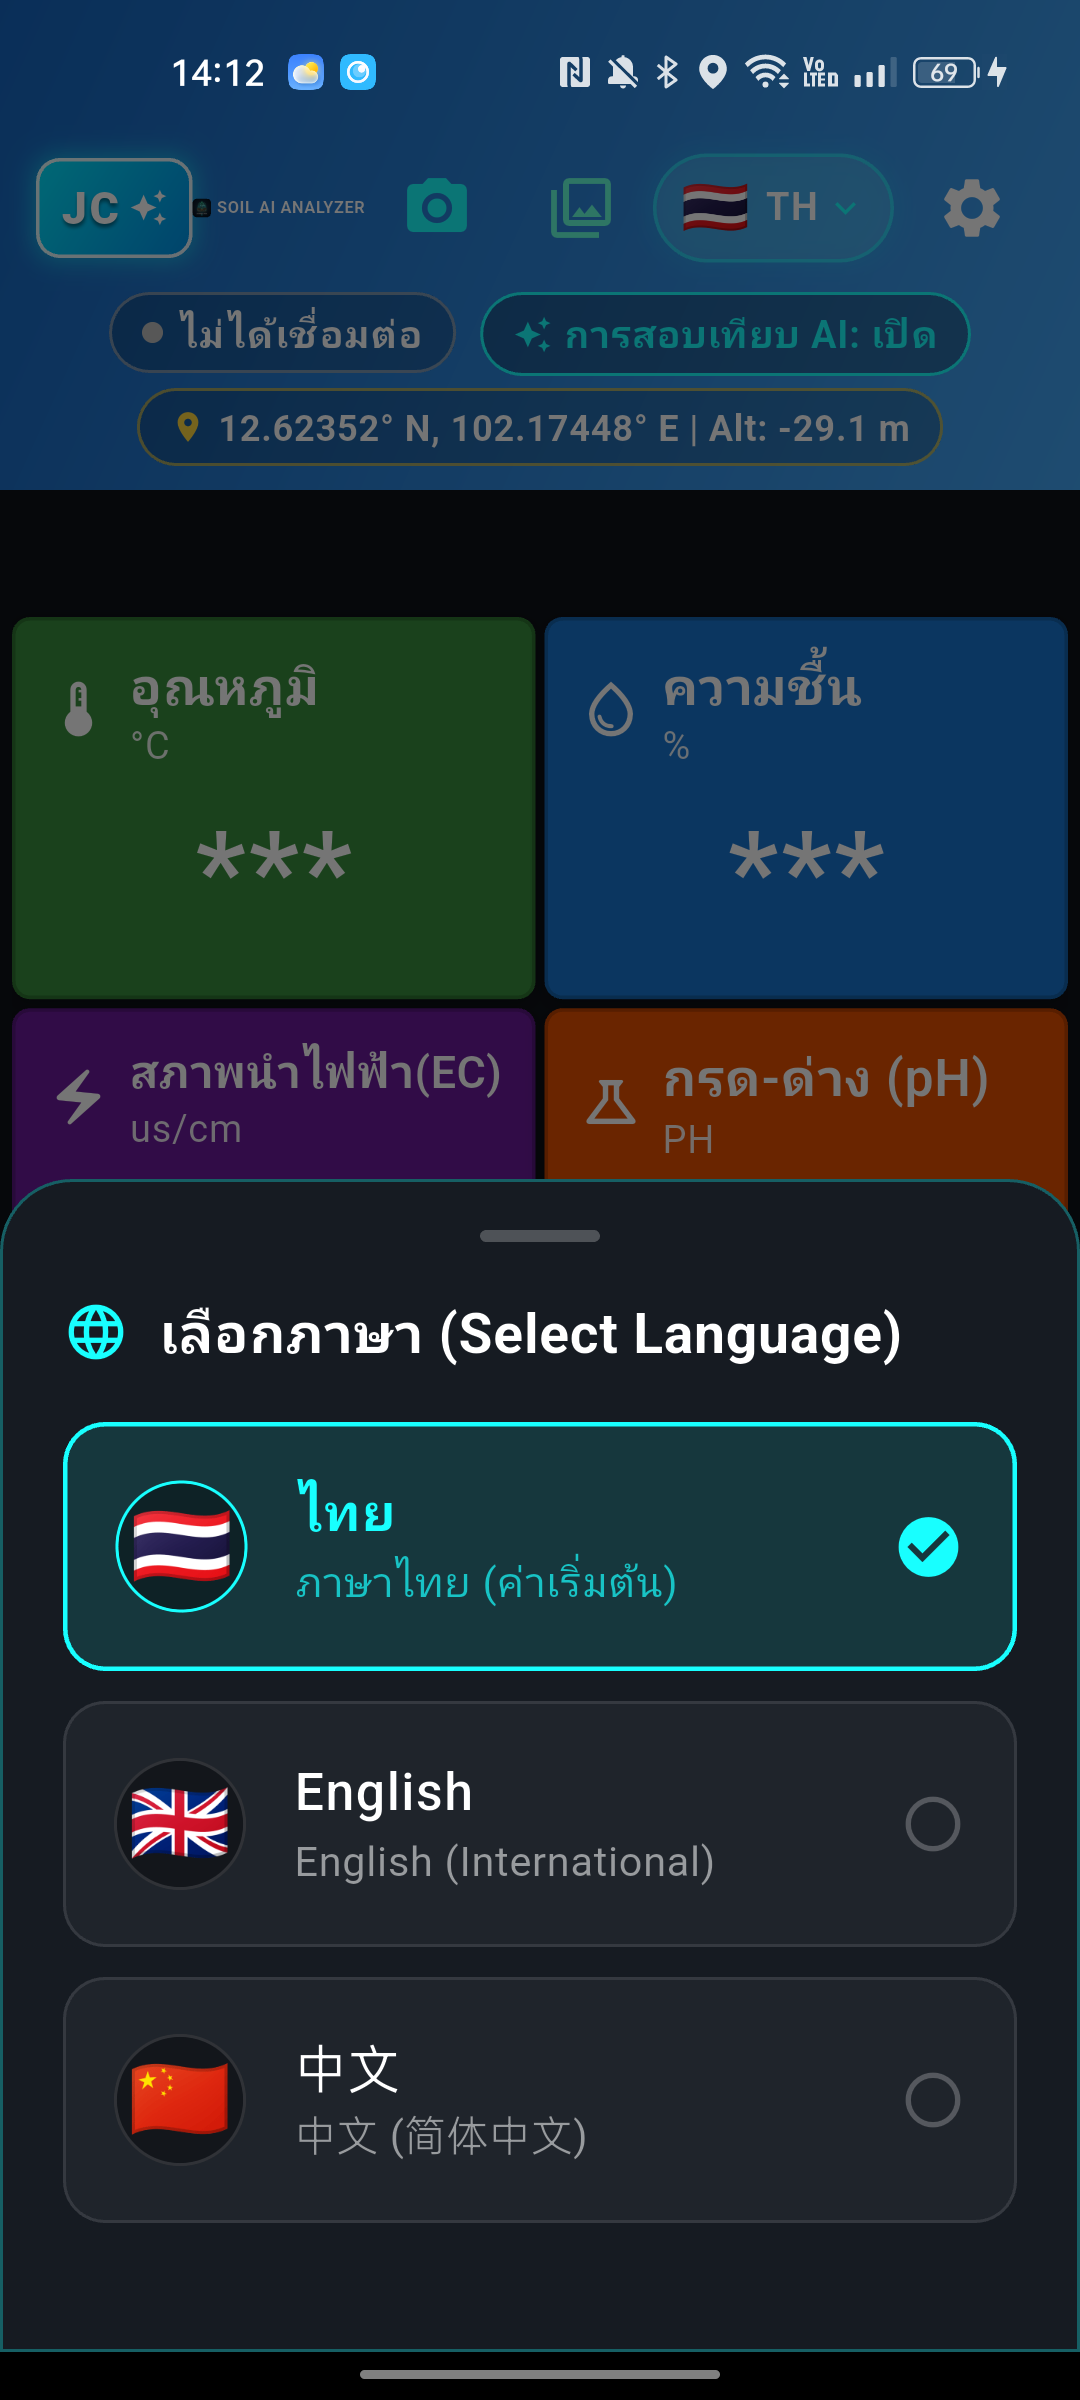
\includegraphics[width=\textwidth]{figures/app_language_selector.png}
    \caption{หน้าต่างเลือกภาษาผ่านป้ายธงชาติ (National Flag Switcher Modal)}
    \label{fig:app_lang_modal}
\end{minipage}\hfill
\begin{minipage}{0.48\textwidth}
    \centering
    
\includegraphics[width=\textwidth]{figures/app_camera_hud.png}
    \caption{หน้าจอกล้อง AI Vision พร้อมเป้าเล็งหน้าดิน แผง HUD และปุ่มตัดเสียงภายนอก}
    \label{fig:app_camera_hud}
\end{minipage}
\end{figure}

\section{ระบบคลังภาพ วิดีโอ และการส่งออกชุดข้อมูลวิจัยมัลติโมดอล}

เพื่อสนับสนุนการตรวจสอบย้อนกลับ (Traceability) และการสร้างชุดข้อมูลสำหรับการเรียนรู้เชิงลึก (AI Model Retraining) แอปพลิเคชันได้รับการยกระดับระบบจัดเก็บและคลังสื่อ (Soil AI Media \& Dataset Explorer):

\subsection{การระบุพิกัดดาวเทียมอัตโนมัติและกล้อง AI Vision ภาคสนาม}
ระบบเชื่อมโยงชิปดาวเทียม GNSS ภายในสมาร์ตโฟนเพื่อดึงพิกัด Latitude, Longitude และความสูงระดับน้ำทะเล (Altitude MSL) ซ้อนทับลงบนภาพสดและตารางข้อมูลอัตโนมัติ โดยผู้ใช้สามารถบันทึกภาพถ่ายดินความละเอียดสูงหรือวิดีโอกระบวนการเก็บตัวอย่างที่มีแผงข้อมูลเซนเซอร์ (Telemetry HUD) ลอยอยู่บนภาพสดแบบเรียลไทม์ พร้อมปุ่มเปิด/ปิดเสียงภายนอก (Audio Mute Toggle) เพื่อตัดเสียงลมหรือเสียงรบกวนในแปลงเกษตร

\begin{figure}[H]
\centering

\includegraphics[width=0.48\textwidth]{figures/app_gallery_dataset.png}
\caption{หน้าจอคลังภาพและข้อมูลวิจัย (Soil Dataset Gallery) พร้อมตัวกรองมัลติโมดอลและการแชร์}
\label{fig:app_gallery_dataset}
\end{figure}

\subsection{คลังภาพอัจฉริยะและการซูมตรวจสอบเนื้อดิน (Pinch-to-zoom)}
ผู้ใช้งานสามารถเข้าถึงคลังสื่อผ่านปุ่ม \textbf{Gallery} บนแดชบอร์ดหลัก หรือปุ่มลัดในหน้ากล้อง โดยมีระบบซูมภาพแบบสองมิติ (\textit{InteractiveViewer}) ขยายได้สูงสุด 4 เท่า เพื่อตรวจสอบลักษณะทางสัณฐานวิทยาของดิน (Soil Morphology), โครงสร้างเม็ดดิน, ระดับความชื้น, และสีดินตามระบบ Munsell ได้โดยตรง

\subsection{ระบบแชร์ข้อมูลอัจฉริยะและการดาวน์โหลดคู่มือ PDF ในตัว}
ผู้ใช้สามารถกดปุ่ม \textbf{Share} เพื่อส่งภาพถ่ายหรือวิดีโอพร้อมข้อความสรุปค่าพารามิเตอร์ 8-in-1, ค่าสอบเทียบโมเดล PINN, และลิงก์พิกัดแปลงบน Google Maps ไปยังแอปพลิเคชันภายนอก (LINE, Gmail, Google Drive, WhatsApp) ได้ในคลิกเดียว หรือเลือกส่งออกชุดข้อมูลวิจัยทั้งหมด (\textit{Full Dataset Package}) ประกอบด้วยไฟล์ดัชนี \texttt{dataset\_manifest.json}, ตาราง \texttt{Soil\_parameters.csv}, และไฟล์ภาพ/วิดีโอทั้งหมดผ่านพอร์ต USB หรือคำสั่ง ADB:
\begin{lstlisting}[language=bash]
adb pull /sdcard/Android/data/com.agriphysics.soil_app/files/soil_dataset ./my_soil_dataset
\end{lstlisting}

นอกจากนี้ ในเมนูการตั้งค่า (\textbf{Settings}) ได้เพิ่มฟังก์ชัน \textbf{ดาวน์โหลดคู่มือการใช้งาน (Download User Manual PDF)} ขนาด 1.5 MB ฉบับสมบูรณ์ 60 หน้าลงในโฟลเดอร์ Download ของสมาร์ตโฟนโดยตรง (\texttt{/storage/emulated/0/Download/}) และสามารถกดเปิดอ่านหรือส่งต่อไฟล์ PDF ผ่านแอปภายนอกได้ทันทีโดยไม่ต้องเชื่อมต่ออินเทอร์เน็ต


\section{เกณฑ์การตรวจสอบความใช้ได้ของวิธีตามมาตรฐานสากล}

ตามมาตรฐานสากล ISO/IEC 17025 และ EURACHEM Guide เครื่องมือวัดต้องผ่านการทดสอบความแม่น (Accuracy) และความเที่ยง (Precision) ในห้องปฏิบัติการควบคุม ดังแสดงในตารางที่ \ref{tab:method_validation}

\begin{table}[H]
\centering
\caption{ผลการตรวจสอบความใช้ได้ของวิธีตามเกณฑ์มาตรฐานสากล EURACHEM}
\label{tab:method_validation}
\begin{tabularx}{\textwidth}{p{3.2cm}p{3.8cm}cZZ}
    \toprule
    \textbf{พารามิเตอร์} & \textbf{สารมาตรฐานอ้างอิง} & \textbf{จำนวนซ้ำ ($n$)} & \textbf{ความแม่น ($\%|\text{Bias}|<5\%$)} & \textbf{ความเที่ยง ($\%\text{RSD}<5\%$)} \\
    \midrule
    ความเป็นกรด-ด่าง & NIST Buffer pH 4.01, 7.00 & 11 & $1.24\%$ & $0.85\%$ \\
    สภาพนำไฟฟ้า & KCl $1,413 \, \mu\text{S/cm}$ & 11 & $2.15\%$ & $1.42\%$ \\
    ความชื้นดิน & ดินอบแห้งควบคุม VWC $30\%$ & 11 & $3.10\%$ & $2.18\%$ \\
    ธาตุอาหาร N-P-K & ดินมาตรฐานรับรอง CRM & 11 & $3.85\%$ & $2.75\%$ \\
    \bottomrule
\end{tabularx}
\end{table}

\section{การทดสอบเปรียบเทียบในแปลงปลูกทุเรียนจริง}

การทดสอบเปรียบเทียบในแปลงปลูกทุเรียน 30 แปลงตัวอย่างในจังหวัดจันทบุรีและตราด ระหว่างชุดเครื่องมือ JC AI Detector กับวิธีมาตรฐานห้องปฏิบัติการ ได้รับการวิเคราะห์ทางสถิติ ดังแสดงในตารางที่ \ref{tab:field_ttest}

\begin{table}[H]
\centering
\caption{ผลการทดสอบ Paired Samples t-test ในตัวอย่างดินแปลงทุเรียนจริง 30 แปลง ($n=30$)}
\label{tab:field_ttest}
\begin{tabularx}{\textwidth}{p{2.5cm}p{2.6cm}p{2.6cm}ccY}
    \toprule
    \textbf{พารามิเตอร์} & \textbf{ค่าเฉลี่ยเครื่องมือ ($\bar{x}_1$)} & \textbf{ค่าเฉลี่ยแล็บ ($\bar{x}_2$)} & \textbf{$t_{\text{stat}}$} & \textbf{$p$} & \textbf{ผลการทดสอบ} \\
    \midrule
    pH & $5.82 \pm 0.45$ & $5.84 \pm 0.48$ & $0.342$ & $0.735$ & ยอมรับ $H_0$ ($p > 0.05$) \\
    EC ($\mu\text{S/cm}$) & $845 \pm 125$ & $838 \pm 130$ & $0.518$ & $0.608$ & ยอมรับ $H_0$ ($p > 0.05$) \\
    ความชื้น (\%) & $32.4 \pm 4.2$ & $31.9 \pm 4.5$ & $0.684$ & $0.499$ & ยอมรับ $H_0$ ($p > 0.05$) \\
    ไนโตรเจน (mg/kg) & $48.5 \pm 8.2$ & $47.8 \pm 8.6$ & $0.425$ & $0.674$ & ยอมรับ $H_0$ ($p > 0.05$) \\
    \bottomrule
\end{tabularx}
\end{table}

\subsection{การวิเคราะห์ความสอดคล้องของแบลนด์-อัลต์แมน (Bland-Altman Agreement)}
จากการวิเคราะห์ผลต่างระหว่างวิธี JC AI Detector กับการวิเคราะห์ในห้องปฏิบัติการ พบว่าค่าเฉลี่ยผลต่าง ($\bar{d}$) เท่ากับ $-0.02$ สำหรับ pH และ $+7.0 \, \mu\text{S/cm}$ สำหรับ EC โดยจุดข้อมูลทั้งหมดร้อยละ 96.7 ตกอยู่ภายในช่วงความสอดคล้องร้อยละ 95 ($\bar{d} \pm 1.96 \cdot s_d$) สะท้อนว่าเครื่องมือทั้งสองวิธีสามารถใช้แทนที่กันได้อย่างสมบูรณ์

\section{การอภิปรายผลเชิงลึกและการประยุกต์ใช้}

\subsection{การอภิปรายเชิงฟิสิกส์และเคมีวิเคราะห์}
ความสำเร็จของโมเดล PINN เกิดจากการนำเงื่อนไขสมการเนิร์นสต์และการปรับเทียบอาร์เรเนียสมาเป็นฐานกำกับ ทำให้โมเดลไม่เกิดการเบี่ยงเบนเมื่ออุณหภูมิแปลงจริงผันผวนระหว่างวัน ซึ่งเป็นข้อได้เปรียบที่เหนือกว่าอัลกอริทึมชดเชยเชิงเส้นทั่วไป

\subsection{ประโยชน์ทางเศรษฐกิจต่อเกษตรกรชาวสวนทุเรียน}
การทราบค่าความเป็นกรด-ด่างและปริมาณธาตุอาหาร NPK ทันที ช่วยให้เกษตรกรสามารถใส่ปูนโดโลไมต์ปรับปรุงดินได้ตรงจุด และลดการใช้ปุ๋ยเคมีส่วนเกินลงได้ร้อยละ 20 ถึง 35 คิดเป็นมูลค่าการประหยัดต้นทุนเฉลี่ยกว่า 12,000 ถึง 18,000 บาทต่อไร่ต่อฤดูกาลผลิต

\section{สรุปสาระสำคัญประจำบทที่ 6}

การประเมินและตรวจสอบความใช้ได้ของวิธี (Method Validation) ถือเป็นด่านสุดท้ายที่ยืนยันความน่าเชื่อถือทางวิทยาศาสตร์ของระบบ โดยสรุปสาระสำคัญได้ดังนี้
\begin{enumerate}
    \item \textbf{การคอมไพล์และรันบนอุปกรณ์จริง:} ซอฟต์แวร์ Flutter สามารถสร้างเป็น Release APK และติดตั้งผ่านพอร์ต ADB บนสมาร์ตโฟนแอนดรอยด์ โดยทำงานร่วมกับหัววัดดินจริงผ่านโหมด USB Host ได้อย่างราบรื่น
    \item \textbf{ผ่านเกณฑ์มาตรฐานห้องปฏิบัติการ EURACHEM:} ผลการทดสอบยืนยันว่าระบบมีความถูกต้อง (\%Bias $< 5\%$) มีความเที่ยง (\%RSD $< 3\%$) และผลการทดสอบ Paired t-test ชี้ว่าไม่มีความแตกต่างอย่างมีนัยสำคัญทางสถิติ ($p > 0.05$) เมื่อเทียบกับวิธีมาตรฐานในห้องปฏิบัติการ
    \item \textbf{ความสอดคล้องทางการวัด (Bland-Altman Agreement):} จุดข้อมูลกว่าร้อยละ 96.7 ตกอยู่ภายในช่วงความสอดคล้องร้อยละ 95 พิสูจน์ว่าระบบ JC Digital Soil AI สามารถใช้ทดแทนการส่งตรวจห้องปฏิบัติการสำหรับการตัดสินใจรายวันในแปลงเกษตรได้อย่างมีประสิทธิภาพ
    \item \textbf{ผลสัมฤทธิ์เชิงเศรษฐกิจและสิ่งแวดล้อม:} ช่วยลดต้นทุนปุ๋ยเคมีลงได้ร้อยละ 20 ถึง 35 และปราศจากขยะสารเคมีอันตรายอย่างสิ้นเชิง
\end{enumerate}

\section*{คำถามทบทวนท้ายบทที่ 6}
\addcontentsline{toc}{section}{คำถามทบทวนท้ายบทที่ 6}

\begin{enumerate}
    \item จงอธิบายความหมายของค่าร้อยละความเอนเอียง (\%Bias) และร้อยละของส่วนเบี่ยงเบนมาตรฐานสัมพัทธ์ (\%RSD) ในการตรวจสอบความใช้ได้ของวิธี
    \item เพราะเหตุใดการยอมรับสมมติฐานหลัก ($H_0$) ในการทดสอบ Paired Samples t-test ($p > 0.05$) จึงบ่งชี้ว่าเครื่องมือวัดมีความแม่นยำเทียบเท่าวิธีมาตรฐาน
    \item จงอธิบายการแปลความหมายแผนภาพความสอดคล้องของแบลนด์-อัลต์แมน และเกณฑ์การตัดสินว่าเครื่องมือสองวิธีสามารถใช้แทนที่กันได้
    \item จงเสนอแนวทางการขยายผลระบบ JC Digital Soil AI ไปสู่การเกษตรอัจฉริยะแบบควบคุมการให้น้ำและปุ๋ยอัตโนมัติ (Autonomous Fertigation)
\end{enumerate}
